\section{Dynamic network analysis}

  \subsection{Discretisation of data}
  
    Because the messages are posted on this forum virtually every minute the information about them might be considered as being continuous in time. In order to study the evolution of the network in time, there is a need to define discrete time intervals that will split the network in parts. Networks that are dynamic are called longitudinal networks.

  \subsection{Collaborative Similarity}
    
    My supervisor, dr Jarosław Kwapień, suggested that it may be a good idea to explore and look at the \emph{user-message network} from the other angle. Ming-Sheng Shang \textit{et al.} have proposed a new index called \emph{collaborative similarity}, to quantify the diversity of tastes based on the collaborative selection.\cite{Shang2010} This newly proposed index sounds promising for the data under analysis in this thesis. If I can find that the user selection is highly clustered---i.e. not that much diverse---then I will be able to easily identify main groups of users.
    
    \subsubsection{The concept}
    
      Figure \ref{fig:cs_network} illustrates a small bipartite network that consists of six users and eight objects. The degree of user $i$, denoted by $k_i$, is defined as the number of objects connected to $i$. Analogously, the degree of object $\alpha$, denoted by $d_\alpha$, is the number of users connected to $\alpha$. For example, as shown in figure \ref{fig:cs_network}, $k_i = d_\alpha = 3$. The density function, $p(k)$, is the probability that a randomly selected user is of degree $k$, while the cumulative function, $P(k)$, denotes the probability that a randomly selected user is of degree no less than $k$.
      \begin{figure}[h]
        \centering
        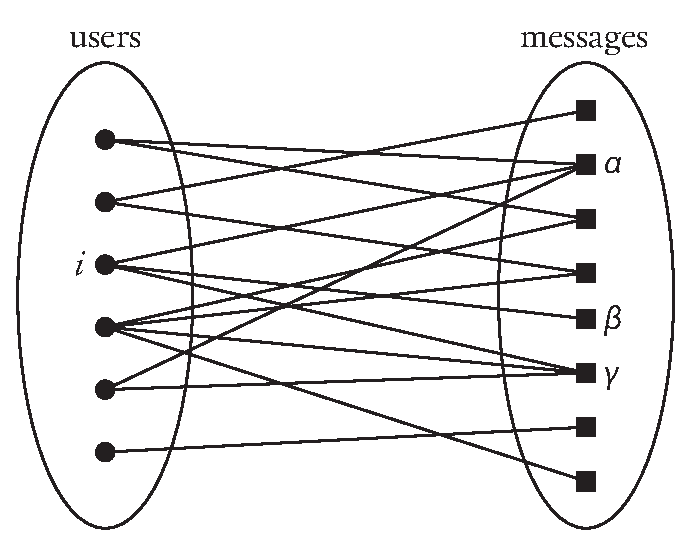
\includegraphics[width=0.6\textwidth]{chapters/03_implementation/cs_network}
        \caption{Small user-message bipartite network.}
        \label{fig:cs_network}
      \end{figure}
      
      The \emph{nearest neighbors’ degree} for user $i$, denoted by $d_{nn}(i)$, is defined as the average degree over all the objects connected to $i$. For example, as shown in figure \ref{fig:cs_network},
      \begin{equation}
        d_{nn}(i) = \frac{d_\alpha + d_\beta + d_\gamma}{3} = \frac{7}{3}\mbox{.}
      \end{equation}

      The degree-dependent nearest neighbors’ degree, $d_{nn}(k)$ is the average nearest neighbors’ degree over all the users of degree $k$, that is,
      \begin{equation}
        d_{nn}(k) = \langle d_{nn}(i) \rangle_{k_i=k}\mbox{.}
      \end{equation}

      Corresponding definitions for objects, say $p(d)$, $P(d)$, $k_{nn}(\alpha)$ and $k_{nn}(d)$, are similar and thus omitted here.
      
      The traditional clustering coefficient\cite{WattsStrogatz1998} cannot be used to quantify the clustering pattern of a bipartite network since it always give a zero value. Lind et al.\cite{LindGonzalezHerrmann2005} proposed a variant counting the rectangular relations instead of triadic clustering, which can be applied to general bipartite networks. However, this letter aims at a special class of bipartite networks, and thus we propose a new index to characterise the clustering selections\footnote{Here the term \textquote{clustering} describes the fact that a user's selections are usually very similar to each other, and may belong to a few clusters or communities according to the standard clustering analysis or community detection.} resulted from the collaborative interests of users. A standard measure of object similarity according to the collaborative selection is the \emph{Jaccard similarity}.\cite{Jaccard1901}
      \begin{equation}
        s_{\alpha\beta} = \frac{\Gamma_\alpha \cap \Gamma_\beta}{\Gamma_\alpha \cup \Gamma_\beta}\mbox{,}
      \end{equation}
      where $\Gamma_\alpha$ and $\Gamma_\beta$ are the sets of neighbouring nodes of $\alpha$ and $\beta$, respectively. Obviously, $s_{\alpha\beta} = s_{\beta\alpha}$ and $0 \leq s_{\alpha\beta} \leq 1$ for any $\alpha$ and $\beta$. For example, as shown in figure \ref{fig:cs_network}, $s_{\alpha\beta} = s{\beta\gamma} = \sfrac{1}{3}$ and ${\alpha\gamma} = \sfrac{1}{2}$. The collaborative similarity of user $i$ is then defined as the average similarity between $i$'s selected objects:
      \begin{equation}
        C_u(i) = \frac{1}{k_i(k_i-1)} \sum_{\alpha\neq\beta} s_{\alpha\beta}\mbox{,}
      \end{equation}
      where $\alpha$ and $\beta$ run over all $i$'s neighbouring objects. For example, as shown in figure \ref{fig:cs_network}, the collaborative similarity of user $i$ is $C_u(i) = \sfrac{7}{18}$. According to the definition, a user whose collections are very similar to each other will have high collaborative similarity. For example, a user who only watches science fiction movies is probably of higher collaborative similarity than the one who has very diverse interests of movies. The user collaborative similarity of the whole network is defined as
      \begin{equation}
        C_u = \frac{1}{N\prime} \sum_{i} C_u(i)\mbox{,}
      \end{equation}
      where $i$ runs over all users with degrees larger than $1$ and $N\prime$ denotes the number of these users. The degree-dependent collaborative similarity, $C_u(k)$, is defined as the average collaborative similarity over all the $k$-degree users. Corresponding definitions for objects are as following:
      \begin{equation}
        C_o(\alpha) = \frac{1}{d_\alpha(d_\alpha-1)} \sum_{i\neq j} s_{ij}\mbox{,}
      \end{equation}
      where $s_{ij} = \left| \frac{\Gamma_i \cap \Gamma_j}{\Gamma_i \cup \Gamma_j} \right|$ is the Jaccard similarity between users $i$ and $j$ and:
      \begin{equation}
        C_o = \frac{1}{M\prime} \sum_\alpha C_o(\alpha)\mbox{,}
      \end{equation}
      where $M\prime$ denotes the number of objects with degrees larger than $1$. $C_o(d)$ is the average collaborative similarity over all the $d$-degree objects.
      
    \subsubsection{Results}
    
      \begin{table}[h]
        \begin{tabularx}{\textwidth}{|C{1.1}|C{0.95}|C{0.95}|C{1}|C{1}|C{1}|C{1}|C{1}|C{1}|C{1}|} \hline
          \rowcolor[gray]{0.75} \textbf{Bucket} & $N$ & $M$ & $E$ & $\langle k \rangle$ & $\langle d \rangle$ & $C_u$ & $\bar s_m$ & $C_m$ & $\bar s_u$ \\\hline
$1$ & $193$ & $2616$ & $29560$ & $78.02$ & $5.76$ & $0.1608$ & $0.1046$ & $0.1278$ & $0.1453$ \\\hline
$11$ & $417$ & $3647$ & $55201$ & $68.54$ & $7.84$ & $0.1376$ & $0.0955$ & $0.1182$ & $0.1148$ \\\hline
$21$ & $609$ & $3787$ & $73964$ & $62.79$ & $10.10$ & $0.1253$ & $0.0936$ & $0.1167$ & $0.1028$ \\\hline
$31$ & $718$ & $4027$ & $89545$ & $63.74$ & $11.37$ & $0.1235$ & $0.0926$ & $0.1166$ & $0.0986$ \\\hline
$41$ & $942$ & $4247$ & $93741$ & $55.60$ & $12.33$ & $0.1070$ & $0.0860$ & $0.1047$ & $0.0857$ \\\hline
$51$ & $1318$ & $4622$ & $118121$ & $51.71$ & $14.75$ & $0.0975$ & $0.0812$ & $0.0995$ & $0.0768$ \\\hline
$61$ & $1966$ & $5232$ & $191560$ & $54.71$ & $20.56$ & $0.0988$ & $0.0849$ & $0.1033$ & $0.0747$ \\\hline
$71$ & $1701$ & $5095$ & $89352$ & $52.53$ & $17.54$ & $0.0975$ & $0.0800$ & $0.0996$ & $0.0741$ \\\hline
$81$ & $1905$ & $5090$ & $91795$ & $48.19$ & $18.03$ & $0.0932$ & $0.0787$ & $0.0985$ & $0.0711$ \\\hline
$91$ & $1680$ & $4774$ & $77094$ & $45.89$ & $16.15$ & $0.0900$ & $0.0775$ & $0.0935$ & $0.0736$ \\\hline
$101$ & $1817$ & $5544$ & $105478$ & $58.05$ & $19.03$ & $0.1096$ & $0.0867$ & $0.1103$ & $0.0799$ \\\hline
$111$ & $1743$ & $4989$ & $81130$ & $46.55$ & $16.26$ & $0.0918$ & $0.0777$ & $0.0961$ & $0.0716$ \\\hline
$121$ & $1706$ & $4900$ & $81357$ & $47.69$ & $16.60$ & $0.0968$ & $0.0784$ & $0.1000$ & $0.0755$ \\\hline
$131$ & $1994$ & $5562$ & $104444$ & $52.38$ & $18.78$ & $0.0986$ & $0.0796$ & $0.1011$ & $0.0732$ \\\hline
$141$ & $2080$ & $5250$ & $94994$ & $45.67$ & $18.09$ & $0.0915$ & $0.0757$ & $0.0962$ & $0.0712$ \\\hline        \end{tabularx}
        \caption{The basic properties of every 10th data bucket.}
        \label{tab:cs_properties}
      \end{table}

      Table \ref{tab:cs_properties} summarises basic statistics of selected data buckets. $N$, $M$ and $E$ denote the number of users, messages and edges connecting them, respectively. $\langle k \rangle$ and $\langle d \rangle$ are the average user degree and average message degree. $C_u$ and $C_m$ are the average collaborative similarity for users and messages, and for comparison, $\bar s_m$ and $\bar s_u$ are the average similarities over all message pairs and over all user pairs, respectively. The user selection is considered to be poorly clustered (i.e., more diverse) because the condition for that is $C_u \gg \bar s_m$ whereas $C_u$ is the same order of magnitude as $\bar s_m$. Unfortunately, this basically means that it will not be easy to identify groups of users that may have formed in this message board and I had to abandon this somewhat interesting index. Figure \ref{fig:cs_cusm} show the way $C_u$ and $\bar s_m$ were changing over time. In no bucket, $C_u$ was much greater than $\bar s_m$ and even in bucket 84 they were pretty close to each other: $0.0746$ vs $0.0683$ respectively.
      \begin{figure}[H]
        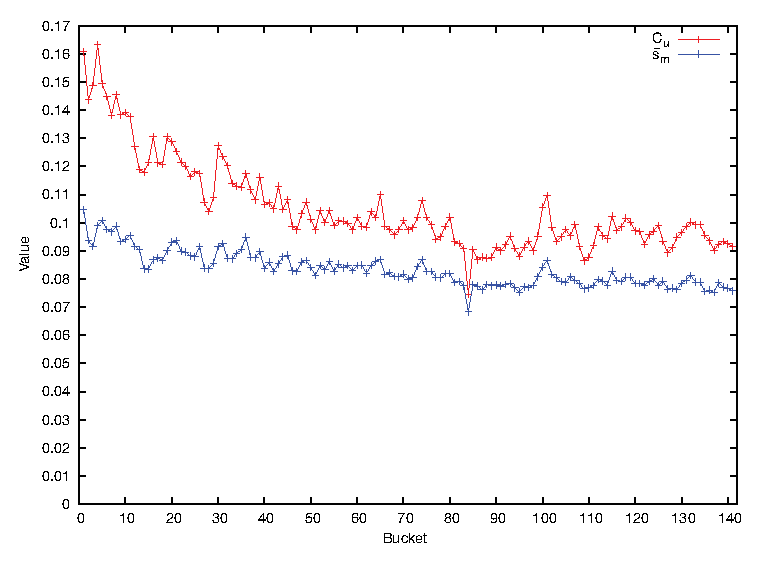
\includegraphics[width=\textwidth]{chapters/03_implementation/C_us_m}
        \caption{Changes of $C_u$ and $\bar s_m$ over time.}
        \label{fig:cs_cusm}
      \end{figure}

  \subsection{Motifs}
  
    \subsubsection{Introduction}
      
      One of the methods that I was sure will bring up some groups of users was the motif discovery within the network. It was found that real world network often feature recurrent sub-graphs or patterns. \emph{Motifs} are sub-graphs that repeat themselves in the network or even in networks of the same type. Indeed, motifs are of notable importance largely because they may reflect functional properties. They have recently gathered much attention as a useful concept to uncover structural design principles of complex networks.\cite{MasoudiSchreiberKashani2012}
      
      Network motifs were at first defined systematically in \emph{Escherichia coli}, where they were detected as patterns that occurred in the transcription network much more often than would be expected in random networks.\cite{MiloAlon2002} The exact same motifs have been later found in other organisms, ranging from other bacteria\cite{ManganZaslaverAlon2003,Eichenberger2004} and yeast\cite{MiloAlon2002, Lee2002}, to plants\cite{Saddic2006} and animals\cite{Boyer2005}. Motif discovery have been the most successful in biological networks, most likely because they were the most studied at the time---especially the transctiption networks. I will not explain many details about the motifs, because this is a complicated matter and already has been discussed and reviewed thoroughly.\cite{Alon2007}
      
    \subsubsection{Motif discovery}
      
      Although network motifs may provide a deep insight into the network's functional abilities, their detection is computationally challenging. Because of that, I have decided to only concentrate on the most basic, triangle motifs, that I have discovered using not very sophisticated algorithm conjoining two users sharing similar opinions about particular brands, hoping that this approach will lead to some interesting opportunities. This also allowed me to map the bipartite network I was working on so far to a regular network built on a set of users exchanging opinions only. Because I have already joined users with brands they were discussing based on the opinion being positive, negative or neutral, the only step required to obtain these triangles was to link users with matching opinions. 
      
      First, the algorithm builds a bipartite network with users and opinions about particular brands. Edges (solid lines) represent the opinion the user has about the product. It is not possible to have more than one edge between the nodes, because all opinions about the brand users may have are averaged and only this average number is taken into account during network creation. When the network is ready, algorithm finds user nodes having edges to the same brand nodes and links them together (dashed lines). The final step involves deletion of initial edges along with brand nodes resulting in non-bipartite network consisting of user nodes only. Figure \ref{fig:cs_motifs} illustrates steps taken by the algorithm.
      \begin{figure}[h]
        \centering
        \begin{subfigure}[b]{0.3\textwidth}
          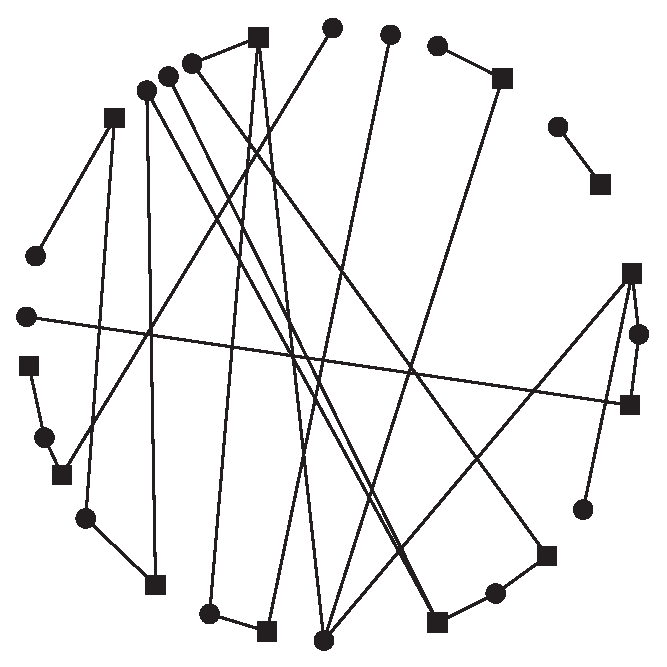
\includegraphics[width=\textwidth]{chapters/03_implementation/cs_motif_1}
          \caption{Step 1.}
        \end{subfigure}
        \quad
        \begin{subfigure}[b]{0.3\textwidth}
          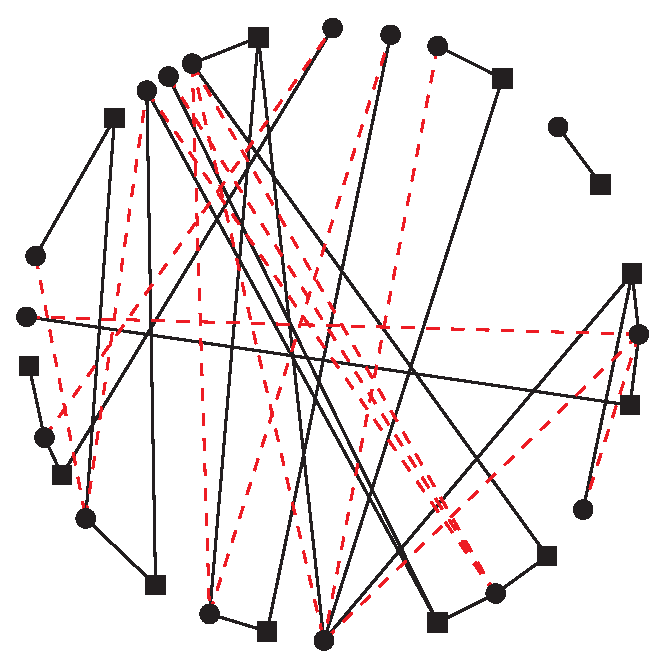
\includegraphics[width=\textwidth]{chapters/03_implementation/cs_motif_2}
          \caption{Step 2.}
        \end{subfigure}
        \quad
        \begin{subfigure}[b]{0.3\textwidth}
          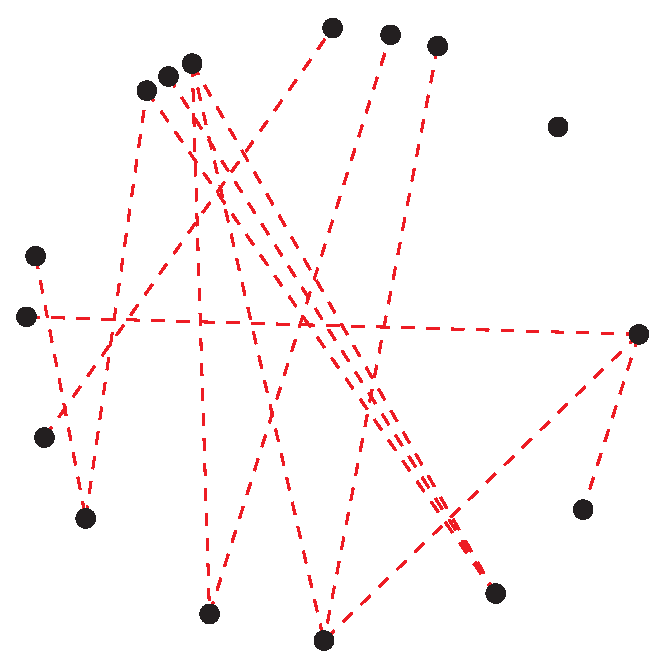
\includegraphics[width=\textwidth]{chapters/03_implementation/cs_motif_3}
          \caption{Step 3.}
        \end{subfigure}
        \caption{Algorithms steps.}
        \label{fig:cs_motifs}
      \end{figure}
      
      After the algorithm has finished mapping bipartite network to non-bipartite network, it is possible to check new network properties, such as the number of connected components which may be significantly different than before.